\section{Algorthm}
\subsection{Detailed Routing Algorthm Analysis}

Conventional framework of detailed routing algorithm we employ follows a structured flow, as illustrated in Algorithm 1. 
Given the global routing results of the benchmarks (e.g..def and.guides files), we perform a track assignment step following the method described in [11], aligning all nets to predefined routing tracks. 
This preprocessing phase extracts and constructs essential data structures, such as routing grids, net objects, and guide constraints, which serve as inputs to the detailed routing engine. 
The ultimate goal is to produce a DRC-clean routing result with full connectivity, starting from these coarse global routing guides.

%%eg [11]M.-P. Wong, W.-H. Liu, and T.-C. Wang, “Negotiation-based track assignment considering local nets,” in Proc. 21st Asia South Pac. Design Automat. Conf. (ASP-DAC), Macau, China, 2016, pp. 378–383.

\begin{algorithm}[hpt]
\caption{Detailed Routing Flow}
\label{alg:detail_routing_algorithm}
\begin{algorithmic}[1]
\Statex \textbf{Input:} base-data structure, global routing guides
\Statex \textbf{Output:} full connected nets
\STATE \text{InitDb()}, \text{InitPreRouteNet()}

\WHILE{$iter < maxIter$}
    \STATE \text {$drcNets \gets [net_{i}: while$ $ net_{i} \in Nets,$$if$ $net_{i}.drcScore \neq 0]$}
    \WHILE{$\text{$net$} \in \text{$drcNets$}$}
        \STATE $\text{$ucPins$} \gets \text{$GetPins(net)$}$
        \WHILE {$ucPins \neq \emptyset$}
            \STATE $\text{$tpin$} \gets \mathop{\arg\max}\limits_{pin \in ucPins} \text{$pin.cost$}$
            \STATE $\text{$cPins$} \gets \text{$cPins$} \cup \text{$tPin$}$, $\text{$ucPins$} \gets \text{$ucPins$} \setminus \text{$tPin$}$
            \STATE $\text{$sPin$} \gets \text{GetNextPin(\text{$ucPins$})}$
            \STATE \text{FPGA-OptimizedRoutingKernel($sPin$,$cPins$)}
        \ENDWHILE
    \ENDWHILE
    
    \STATE \text{UpdateDRC()}, \text{UpdateNets()}
\ENDWHILE
\STATE \text{UpdateDb()}
\end{algorithmic}
\end{algorithm}


The detailed routing flow, as depicted in Algorithm 1, comprises multiple sequential phases. Initially, the design database is initialized via InitDb(), and essential nets are pre-routed using InitPreRouteNet(). Following this, nets are evaluated based on their design rule check scores, and those exhibiting violations are prioritized for further processing.
The outer loop (lines 2 to 14) performs iterative rip-up and reroute operations, bounded by a predefined maximum iteration count. In each iteration, the set of nets with non-zero DRC scores is extracted. For each net in drcNets, the set of unconnected pins is identified (line 5). The algorithm proceeds to incrementally connect these pins by repeatedly selecting the pin with the highest routing cost as the current target, moving it to the connected pin set, and identifying the next nearest source pin (lines 6–9).
Routing between the selected source and target pins uses the Optimized Routing kernel, which leverages high-throughput hardware acceleration. This process continues until all pins in the net are connected. After net-level rerouting, the global DRC state and net data structures are updated accordingly . Upon convergence or exhaustion of iterations, a final database update is performed, reflecting the complete routing solution.


\subsection{Routing Kernel and Generating Routing Graphs Algorthm Analysis}
The most popular detailed routing methods, like TritonRoute[?] and Dr. CU[?], are both executed by the maze routing kernel to connect all pins on the nets with minimal cost. 
In the actual computing stage, the nets will first abstracted as grid graphs. Each pin pn is equivalent to a set of vertices Sn located on its position, 
then utilize the priority queue and some heuristic methods to improve the quality and speed.Taking TritonRoute[?] as an example, it uses A* (A-STAR) algorithm to explore the route and sets weight for each node.
The weight is a heuristic function f (x) : f (x) = g(x) + h(x), where the function g(x) is the distance or cost from the starting node to current state x, and the function h(x) defines the estimated distance or cost from current state x to the end node. 
We call the function value of f (x) the f value. 


\begin{algorithm}[hpt]
\caption{FPGA-Optimized Routing Kernel Algorithm}
\label{alg:FPGA in A* algorithm}
\begin{algorithmic}[1]
\Statex \textbf{Input:} source pin $s$, target pins $\{t_1, \dots, t_n\}$
\Statex \textbf{Output:} minimum-cost routing paths
\Statex \textbf{Prepare:} priority queue $Q$, cost map $T$, flag map $F$, graph batch $G$ $\{G_1, ..., G_N\}$, direction set $D$ $\{E, W, N, S, U, D\}$ in BRAM

\STATE Initialize $N$ grid maps in BRAM
\FOR {$G_k \in G$ \textbf{in parallel}}
    \State \textbf{set} $Q^{(k)}$, $T^{(k)}(v) \gets \infty$, $F^{(k)}(v) \gets 0, \forall v$; $T^{(k)}(s) \gets 0$
    \WHILE{$Q^{(k)} \neq \emptyset$ }
        \STATE $v \gets \text{MinCost($Q^{(k)}$)}$
        \STATE $if$ $v \in \{t_1,...,t_n\}$ \textbf{break}
        \FOR{$u \in D $ \textbf{in parallel}}
            \State $c \gets T^{(k)}(v) + \Delta(v,u)$
            \IF{$c < T^{(k)}(u)$}
                \State $T^{(k)}(u) \gets c$, $F^{(k)}(u) \gets 1$, $u.parent \gets v$
                \State \text{Update($Q^{(k)}$)}
            \ENDIF
        \ENDFOR
    \ENDWHILE

    \State \text{BackTrack Path}
\ENDFOR
\end{algorithmic}
\end{algorithm}

% \clearpage  % 结束当前页
% \vspace*{0pt}  % 避免覆盖已有内容
\afterpage{  % 当前页结束后执行
\begin{figure*}[!t]
    \centering
    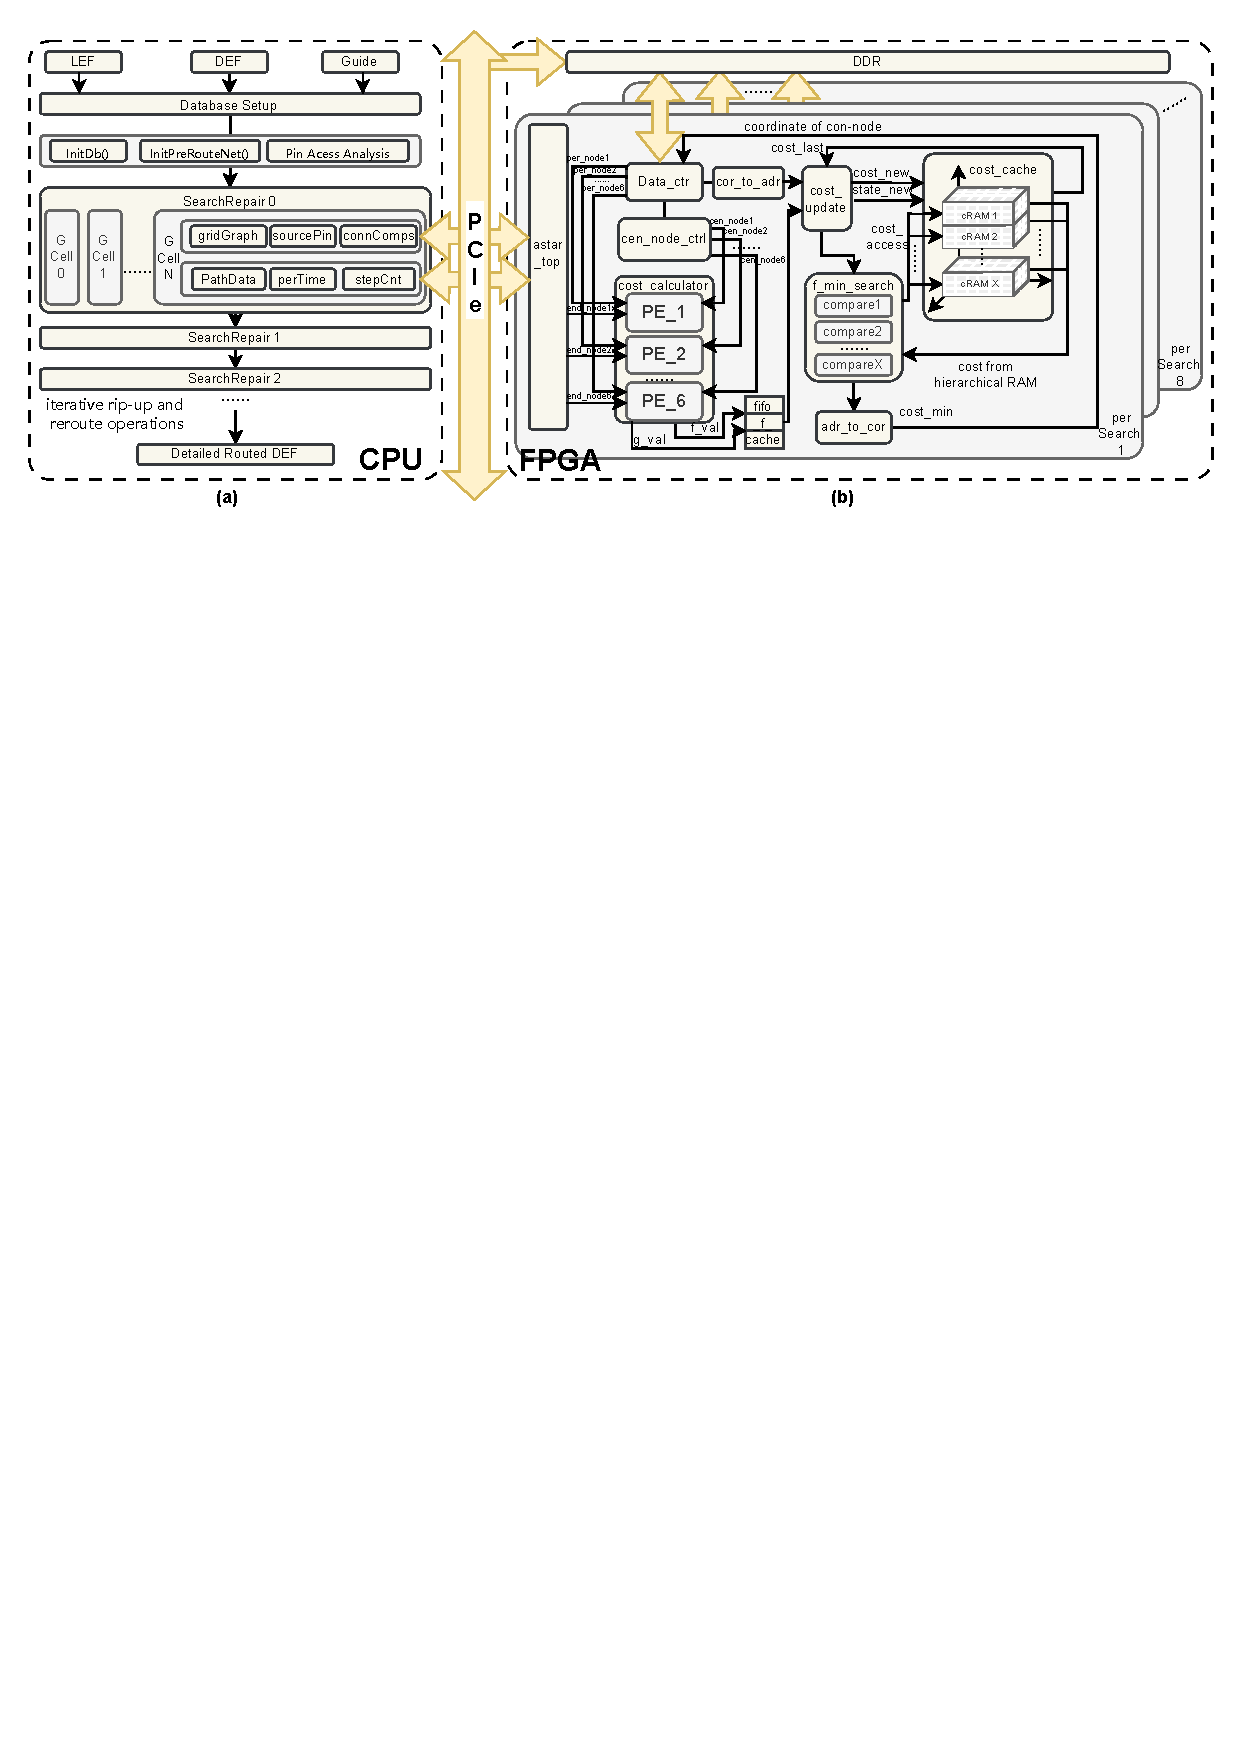
\includegraphics[width=\textwidth]{figures/acceleration/Arch Overview.pdf}
    \caption{The overview structure.(a) The flow of detailed router on GPU.(b) The overview of FPGA acceleration framework.}
    \label{fig:overview} % 标签紧跟标题
\end{figure*}
}

In each round of A* search, we extract the state with the minimum f value from the open list, expand its outer neighbors and check for duplication.
In general, Batched maze routing kernel is executed on a large batch of graphs in the detailed routing stage. There are almost 1,000 ~ 10,000 graphs (nets) in one batch without data dependency between any two graphs, providing a powerful condition for parallelization operation on FPGA to achieve efficient acceleration.

However, the typical maze routing algorithm should be modified to adapt the property of FPGA,as Algorithm 2 shows.
The grid map is initialized in the memory and the start and end nodes are sent to the design so it can start solving the map.
The priority queue Q, the temporary cost set T, and the vertices' state set F used in the hardware-optimized maze routing algorithm are also implemented on hardware.
At the outer level, multiple routing graphs are processed concurrently, exploiting batch-level parallelism with thousands of nets in BRAM.
At the inner level, for each graph, neighbour expansions across multiple directions are executed in parallel to accelerate wavefront propagation.
This fine-grained directional parallelism, combined with hardware-managed cost updates and queue operations, enhances routing throughput on FPGA.

In the process of generating routing diagram, take TritonRoute[?] as an example, through the breadth-first search (BFS) path planning method of extending and updating wavefront, 
the wavefront is dynamically generated and explored in six directions, southeast, northwest and upper, lower, and lower, to gradually update the cost information of each node to realize the path between the target point and the starting point.
It can also be deployed on FPGAs for acceleration through full parallelism and data processing optimization.


%route Split the whole process

%wiring (A* search algorithm is arranged on the FPGA convolution kernel).

%Disassemble and redistribute (compare with the global database, modify the weight), and iterate.

%and the separation of other steps of DRC.

%Processing of database.


% % \subsection{Architecture Design Overview}
% We propose a Mamba accelerator with reconfigurable architecture, \we, with reconfigurable computing units (CUs) and processing elements (PEs).
% \we is a reconfigurable architecture whose instructions are all 64-bit, and contains 16 32-bit general-purpose Registers (Regs) and 16 32-bit Constant Registers (CRegs).
% \we consists of four main parts: instruction processing, normalization unit, on-chip buffer, and computing engine, as depicted in Figure.~\ref{fig:architecture} left.

% \textbf{Instruction Processing.}
% The instruction processing consists of two parts: instruction fetch and instruction decode. 
% The instruction fetch unit fetches instructions from global memory and stores them in the instruction buffer. 
% Then, the instruction decode unit reads instructions sequentially from the buffer and decodes them.
% As shown in Figure~\ref{fig:isa}, the instruction set architecture (ISA) includes linear (\texttt{LIN}), convolution (\texttt{CONV}), normalization (\texttt{NORM}), element-wise multiplication (\texttt{EWM}), element-wise addition (\texttt{EWA}), exponential function (\texttt{EXP}), and SiLU (\texttt{SILU}). 
% And \we also provides \texttt{LOAD} and \texttt{STORE} instructions to support moving data between global memory and on-chip buffer.
% After decoding, the instructions are passed through the configure unit to pass configuration information to the following modules.



% % \textbf{On-chip Buffer.}
% % Buffers are strategically placed throughout the architecture to enhance efficiency. 
% % The buffer pool consists of the input buffer, output buffer, and reconfigurable dual-mode buffer. 
% % The configuration unit determines whether the dual-mode cache serves as an input buffer or an output buffer based on different instructions decoded. 
% % Prior to executing computations, the memory access handler reads data from global memory and writes it into the input buffer for use by computational units. 
% % Intermediate results during computation, as well as the final results, are first written into the output buffer and then transferred to global memory via the memory access handler.


% \textbf{Normalization Unit.}
% The layer normalization is a important component that stabilizes range of intermediate values by normalizing layer activation. 
% The normalization unit is responsible for computing the mean and variance of the data. 
% The data is first summarized and accumulated to get the mean and then the variance is calculated.
% Then, data undergoes a linear unit to obtain the normalized result.

% \textbf{Compute Engine.}
% The compute engine is responsible for linear, convolutional, and element-wise computations. 
% It comprises a control unit and a reconfigurable compute units (RCUs). 
% The control unit receives configuration information from configure unit and fetches data from on-chip buffer to RCU.
% When the computation is completed, it notifies the instruction processing pipeline to continue decoding and executing the next instruction. 


% % \begin{table}[!b]
% % \small
% %   \vspace{-10pt}
% %   \caption{Instruction Set Architecture Definition}
% %   \centering
% %   \vspace{-5pt}
% %   \label{tab:isa}
% %   \begin{tabular}{|l|c|c|c|c|c|}
% %     \hline
% %     \multirow{2}{*}{Operation} & \multirow{2}{*}{Opcode} & Input 0  & Input 1 & Input 1 & Output \\
% %     \multirow{2}{*}{} & \multirow{2}{*}{} & Address & Address & Constant & Address\\
% %     \hline
% %     Linear & 3'b000 & $\checkmark$ & $\checkmark$ & $\checkmark$ & $\checkmark$\\ 
% %     \hline
% %     Conv. & 3'b001 & $\checkmark$ & $\checkmark$ & $\times$ & $\checkmark$ \\ 
% %     \hline
% %     Norm. & 3'b010 & $\checkmark$ & $\times$ & $\times$ & $\checkmark$ \\ 
% %     \hline
% %     Ele. Mul. & 3'b100 & $\checkmark$ & $\checkmark$ & $\checkmark$ & $\checkmark$ \\ 
% %     \hline
% %     Ele. Add. & 3'b101 & $\checkmark$ & $\checkmark$ & $\checkmark$ & $\checkmark$ \\ 
% %     \hline
% %     Ele. Exp. & 3'b110 & $\checkmark$ & $\times$ & $\times$ & $\checkmark$ \\ 
% %     \hline
% %     Ele. SiLU & 3'b111 & $\checkmark$ & $\times$ & $\times$ & $\checkmark$ \\ 
% %   \hline
% % \end{tabular}
% % % \vspace{-10pt}
% % \end{table}

%  \begin{figure*}[!t]
%   \centering
%   \vspace{-5pt}
%   \includegraphics[width=0.98\textwidth]{figures/method1/architecture.pdf}
%   \vspace{-12pt}
%   \caption{Left: Architecture of \we accelerator. \we mainly consists of an instruction processing, a normalization unit, an on-chip buffer,and a compute engine. Middle: Architecture of reconfigurable processing element and reduction tree in RCU. Right: Four reconfigurable modes of RCU, MM-RCU, EW-RCU, EXP-RCU, and SiLU-RCU.}
%   \vspace{-10pt}
%   \label{fig:architecture}
% \end{figure*}

% \begin{figure}[!t]
%   \centering
%   %\vspace{-15pt}
%   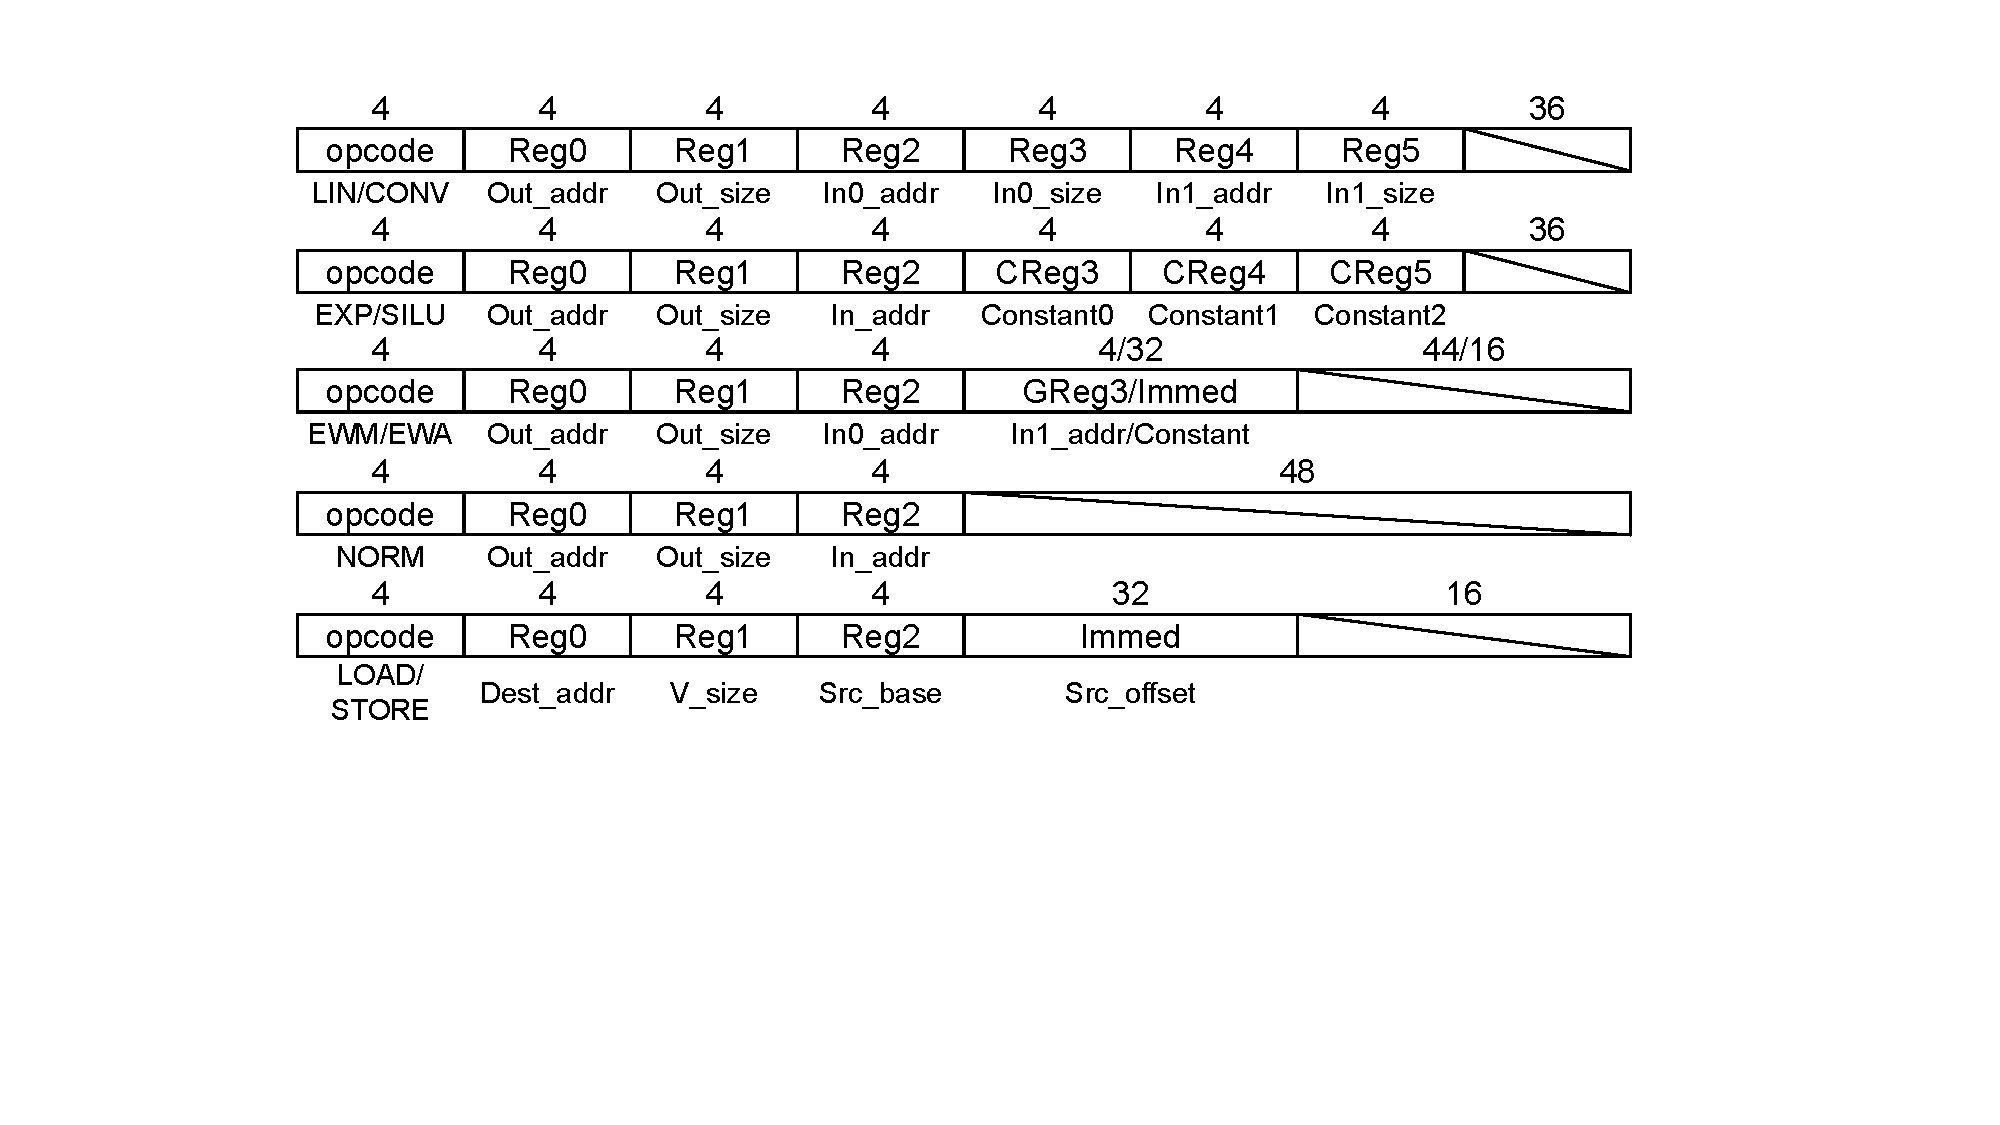
\includegraphics[width=0.48\textwidth]{figures/overview/isa.pdf}
%   \vspace{-18pt}
%   \caption{Instruction set architecture with 16 32-bit general-purpose registers and 16 32-bit constant registers. All instructions are 64-bit.}
%   \vspace{-15pt}
%   \label{fig:isa}
% \end{figure}